\documentclass[tikz,border=10pt]{standalone}
\usepackage{tikz}
\usetikzlibrary{shapes, arrows.meta, positioning, fit, calc, backgrounds, shadows}
\usepackage{amsmath, amssymb}
\usepackage{newtxtext,newtxmath} 

% ==========================================
%  1. 配色定义
% ==========================================
\definecolor{cThreadFill}{RGB}{225, 245, 254}
\definecolor{cThreadDraw}{RGB}{2, 119, 189}
\definecolor{cSyncFill}{RGB}{224, 242, 241}
\definecolor{cSyncDraw}{RGB}{0, 105, 92}
\definecolor{cDataFill}{RGB}{255, 243, 224}
\definecolor{cDataDraw}{RGB}{239, 108, 0}
\definecolor{bgLayerScope}{RGB}{240, 244, 248} 
\definecolor{lineColor}{RGB}{60, 60, 60}       

% ==========================================
%  2. 样式设置 (严格无空行版)
% ==========================================
\tikzset{
    node distance=0.8cm and 0.8cm,
    font=\footnotesize\sffamily,
    % --- 基础块样式 ---
    baseBlock/.style={
        rectangle, thick, rounded corners=3pt,
        align=center,
        drop shadow={opacity=0.1, shadow xshift=1pt, shadow yshift=-1pt}
    },
    % --- 列样式定义 ---
    % Col 1: Namespace/Class
    styleColCtx/.style={
        baseBlock, draw=cSyncDraw, fill=cSyncFill, font=\bfseries\footnotesize,
        text width=3.5cm, minimum height=1.2cm
    },
    % Col 2: Function
    styleColFunc/.style={
        baseBlock, draw=black!40, fill=white, font=\ttfamily\scriptsize,
        text width=4.2cm, minimum height=1.2cm, align=left
    },
    % Col 3: Return Type
    styleColRet/.style={
        baseBlock, draw=cDataDraw, fill=cDataFill, font=\ttfamily\scriptsize,
        text width=3.2cm, minimum height=1.2cm
    },
    % --- 连线样式 ---
    conn/.style={
        draw=lineColor!50, line width=0.8pt,
        -{Latex[length=2mm, width=1.2mm]}
    },
    % --- 背景层样式 ---
    styleScope/.style={
        rectangle, draw=black!10, fill=bgLayerScope,
        inner sep=15pt, rounded corners=5pt
    }
}

\begin{document}
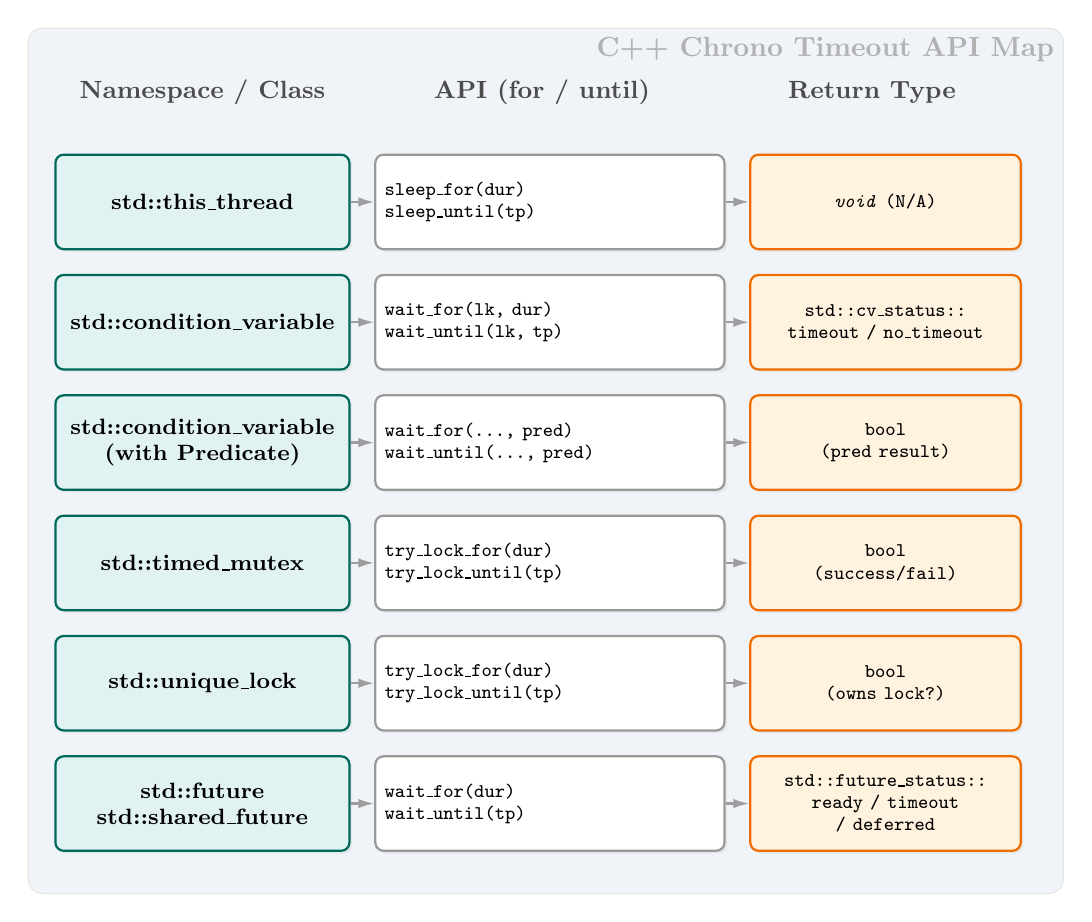
\begin{tikzpicture}

	% =========================================================
	% 3. 表头 (Headers)
	% =========================================================
	\node[font=\bfseries\small, text=black!70] (h1) at (0,0) {Namespace / Class};
	\node[font=\bfseries\small, text=black!70, right=4.5cm of h1.west] (h2) {API (for / until)};
	\node[font=\bfseries\small, text=black!70, right=9.0cm of h1.west] (h3) {Return Type};

	% =========================================================
	% 4. 内容行 (Rows)
	% =========================================================

	% --- Row 1: this_thread ---
	\node [styleColCtx, below=0.5cm of h1] (r1_c) {std::this\_thread};
	\node [styleColFunc, right=0.3cm of r1_c] (r1_f) {sleep\_for(dur)\\sleep\_until(tp)};
	\node [styleColRet, right=0.3cm of r1_f] (r1_r) {\textit{void} (N/A)};

	% --- Row 2: CV (basic) ---
	\node [styleColCtx, below=0.3cm of r1_c] (r2_c) {std::condition\_variable};
	\node [styleColFunc, right=0.3cm of r2_c] (r2_f) {wait\_for(lk, dur)\\wait\_until(lk, tp)};
	\node [styleColRet, right=0.3cm of r2_f] (r2_r) {std::cv\_status::\\timeout / no\_timeout};

	% --- Row 3: CV (predicate) ---
	\node [styleColCtx, below=0.3cm of r2_c] (r3_c) {std::condition\_variable\\(with Predicate)};
	\node [styleColFunc, right=0.3cm of r3_c] (r3_f) {wait\_for(..., pred)\\wait\_until(..., pred)};
	\node [styleColRet, right=0.3cm of r3_f] (r3_r) {bool\\(pred result)};

	% --- Row 4: Timed Mutex ---
	\node [styleColCtx, below=0.3cm of r3_c] (r4_c) {std::timed\_mutex};
	\node [styleColFunc, right=0.3cm of r4_c] (r4_f) {try\_lock\_for(dur)\\try\_lock\_until(tp)};
	\node [styleColRet, right=0.3cm of r4_f] (r4_r) {bool\\(success/fail)};

	% --- Row 5: Unique Lock ---
	\node [styleColCtx, below=0.3cm of r4_c] (r5_c) {std::unique\_lock};
	\node [styleColFunc, right=0.3cm of r5_c] (r5_f) {try\_lock\_for(dur)\\try\_lock\_until(tp)};
	\node [styleColRet, right=0.3cm of r5_f] (r5_r) {bool\\(owns lock?)};

	% --- Row 6: Future ---
	\node [styleColCtx, below=0.3cm of r5_c] (r6_c) {std::future\\std::shared\_future};
	\node [styleColFunc, right=0.3cm of r6_c] (r6_f) {wait\_for(dur)\\wait\_until(tp)};
	\node [styleColRet, right=0.3cm of r6_f] (r6_r) {std::future\_status::\\ready / timeout / deferred};

	% =========================================================
	% 5. 装饰与连线
	% =========================================================
	\foreach \i in {1,...,6} {
			\draw [conn] (r\i_c) -- (r\i_f);
			\draw [conn] (r\i_f) -- (r\i_r);
		}

	% =========================================================
	% 6. 背景层
	% =========================================================
	\begin{scope}[on background layer]
		\node [styleScope, fit=(h1) (r6_r),
			label={[anchor=north east, text=black!30, font=\bfseries]north east:C++ Chrono Timeout API Map}] {};
	\end{scope}

\end{tikzpicture}
\end{document}